\section{Experiments}
\label{sec:exp}

%\JG{please present (1) tasks and metrics, following Table 1 in \citet{wang2018glue}; (2) official test results on the leaderboard (In addition to BERT, we can include other published results, as in Table 1 of \citet{bert2018} plus our official results i.e., 82.2\%; (3) ablation results on dev set, showing the contributions multi-task learning (single-task vs. multi-task),  task reformulation (SAN-answer net, pairwise ranking vs. classification), learning curve of single tasks with and without MLT similar to Figure 4 in \citet{liu2015mtl}, etc.}
\begin{table*}[htb!]
	\begin{center}
		\begin{tabular}{l|l|c|c|c|c|c}
			\hline \bf Corpus &Task& \#Train & \#Dev & \#Test   & \#Label &Metrics\\ \hline \hline
			\multicolumn{6}{@{\hskip1pt}r@{\hskip1pt}}{Single-Sentence Classification (GLUE)} \\ \hline
			CoLA & Acceptability&8.5k & 1k & 1k & 2 & Matthews corr\\ \hline
			SST-2 & Sentiment&67k & 872 & 1.8k & 2 & Accuracy\\ \hline \hline
			\multicolumn{6}{@{\hskip1pt}r@{\hskip1pt}}{Pairwise Text Classification (GLUE)} \\ \hline
			MNLI & NLI& 393k& 20k & 20k& 3 & Accuracy\\ \hline
            RTE & NLI &2.5k & 276 & 3k & 2 & Accuracy \\ \hline
            WNLI & NLI &634& 71& 146& 2 & Accuracy \\ \hline
			QQP & Paraphrase&364k & 40k & 391k& 2 & Accuracy/F1\\ \hline
            MRPC & Paraphrase &3.7k & 408 & 1.7k& 2&Accuracy/F1\\ \hline
			\multicolumn{5}{@{\hskip1pt}r@{\hskip1pt}}{Text Similarity (GLUE)} \\ \hline
			STS-B & Similarity &7k &1.5k& 1.4k &1 & Pearson/Spearman corr\\ \hline

\multicolumn{6}{@{\hskip1pt}r@{\hskip1pt}}{Relevance Ranking (GLUE)} \\ \hline \hline
			QNLI & QA/NLI& 108k &5.7k&5.7k&2& Accuracy\\ \hline \hline
			\multicolumn{6}{@{\hskip1pt}r@{\hskip1pt}}{Pairwise Text Classification} \\ \hline
			SNLI & NLI& 549k &9.8k&9.8k&3& Accuracy\\ \hline
			SciTail & NLI& 23.5k &1.3k&2.1k&2& Accuracy\\ \hline

		\end{tabular}
	\end{center}
%	\lgspace
	\caption{Summary of the three benchmarks: GLUE, SNLI and SciTail.
	}
	\label{tab:datasets}
\lgspace
\end{table*}

We evaluate the proposed {\MNAME} on three popular NLU benchmarks: GLUE \cite{wang2018glue}, Stanford Natural Language Inference (SNLI) \cite{snli2015} and SciTail \cite{scitail}. 
We compare MT-DNN with existing state-of-the-art models including BERT, 
and demonstrate the effectiveness of MTL for model fine-tuning using GLUE and domain adaptation using SNLI and SciTail. 
% analyze the positive impact of multi-task learning with detailed experiments.

%This section presents MT-DNN's multi-task fine-tuning results and domain adaptation results on 11 NLU tasks.

%%%%%%%%%%%%%%%%%%%%%%%%%%%%%%%%%%%%%%%%%
% DATA SETS
%%%%%%%%%%%%%%%%%%%%%%%%%%%%%%%%%%%%%%%%%
%\subsection{Experiment Setup}
%\noindent \textbf{Datasets:} 
\subsection{Datasets}
\label{subsec:dataset}
This section briefly describes the GLUE, SNLI and SciTail datasets, as summarized in Table~\ref{tab:datasets}.
%The detailed description of the GLUE benchmark, SNLI and SciTail is briefly introduced in the following subsections can be found from \cite{wang2018glue, snli2015, scitail} with a brief introduction provided in following subsections. 

The GLUE benchmark is a collection of nine NLU tasks, including question answering, sentiment analysis and textual entailment, and is considered well-designed for evaluating the generalization and robustness of NLU models. 
Both SNLI and SciTail are NLI tasks. 
%We group all 11 tasks into four categories.
% covering a  question answering, sentiment analysis and textual entailment. GLUE challenging yet well designed to compare the generalization and robustness of various NLU models. 

%\subsubsection{Single-Sentence Classification Datasets}
%\label{subsec:ssc}
\paragraph{CoLA} The Corpus of Linguistic Acceptability is to predict whether an English sentence is linguistically “acceptable” or not \cite{cola2018}. %It is formulated as a binary single-sentence classification task.
It uses Matthews correlation coefficient \cite{matthews1975comparison} as its evaluation metric.

\paragraph{SST-2} The Stanford Sentiment Treebank is to determine the sentiment of sentences. % and it is formulated as a binary single-sentence classification task. 
The sentences are extracted from movie reviews
with human annotations of their sentiment \cite{sst2013}. Accuracy is used as its evaluation metric.

%\subsubsection{Text Similarity Datasets}
\paragraph{STS-B}
The Semantic Textual Similarity Benchmark is a collection of sentence pairs collected from multiple data resources including news headlines, video and image captions and NLI data \cite{sts-b2017}. Each pair is human-annotated with a similarity score from 1 to 5, indicating how similar the two sentences are. 
The task is evaluated using two metrics: the Pearson and Spearman correlation coefficients.

%\subsubsection{Relevance Ranking Datasets}
\paragraph{QNLI}
This is derived from the Stanford Question Answering Dataset \citep{rajpurkar2016squad} 
which  has  been converted to a binary classification task in GLUE.
A query-candidate-answer pair is labeled as positive if the candidate contains the correct answer to the query, and negative otherwise. 
In this study, however, we formulate QNLI as a relevance ranking task, where for a given query, its positive candidate answers are considered more relevant, and thus should be ranked higher, than its negative candidates.
%In our experiments, we formulate it as a relevance ranking task and we will show the difference between these two formulations in the following sections. It uses accuracy as its evaluation metric.

%\subsubsection{Pairwise Text Classification Datasets}
%This category consists of 6 GLUE tasks, SNLI and SciTail. 
%All of these tasks use accuracy as the final evaluation metric. 
%However, due to the imbalance property between positive and negative examples, the \textbf{MRPC} and \textbf{QQP} tasks also use F1 score as the final metric, in addition to accuracy.  

\paragraph{QQP}
The Quora Question Pairs dataset is a collection of question pairs extracted from the community question-answering website Quora. The task is to predict whether two questions are semantically equivalent \cite{chen2018quora}. 
As the distribution of positive and negative labels is unbalanced, both accuracy and F1 score are used as evaluation metrics.

\paragraph{MRPC} The Microsoft Research Paraphrase Corpus consists of sentence pairs automatically extracted from online news sources, with human annotations
to label whether a sentence pair is semantically equivalent to the other in the pair \cite{mrpc2005}. 
Similar to QQP, both accuracy and F1 score are used as evaluation metrics.

\paragraph{MNLI}
Multi-Genre Natural Language Inference is a large-scale, crowdsourced entailment classification task \cite{mnli2017}.
%and its premises are collected from a broad range of genre of American English
Given a pair of sentences (i.e., a premise-hypothesis pair), the goal is to predict whether the hypothesis is an \textit{entailment}, \textit{contradiction}, or
\textit{neutral} with respect to the premise. 
The test and development sets are split into in-domain (matched) and cross-domain (mismatched) sets. The evaluation metric is accuracy.

\paragraph{RTE}
The Recognizing Textual Entailment dataset is collected from a series of annual challenges on textual entailment. The task is similar to MNLI, but uses only two labels: \textit{entailment} and \textit{not\_entailment} \cite{wang2018glue}.

\paragraph{WNLI}
The Winograd NLI (WNLI) is a NLI dataset derived from the Winograd Schema dataset \cite{winograd2012}. This is a reading comprehension task. The goal is to select the referent of a pronoun from a list of choices in a given sentence which contains the pronoun.

\paragraph{SNLI}
The Stanford Natural Language Inference (SNLI) dataset contains 570k human annotated sentence pairs, in which the premises are drawn from the captions of the Flickr30 corpus, and hypothesis are manually annotated \cite{snli2015}. %The evaluation metric is accuracy as well.
This is the most widely used entailment dataset for NLI.
The dataset is used only for domain adaptation in this study.

\paragraph{SciTail}
This is a textual entailment dataset derived from a science question answering (SciQ) dataset \cite{scitail}. The task involves assessing whether a given premise entails a given hypothesis.  
Different from other entailment datasets mentioned above, the hypotheses in SciTail are created from science questions and the corresponding answer candidates, and premises from relevant web sentences retrieved from a large corpus. As a result, these sentences are linguistically challenging and the lexical similarity of premise and hypothsis is often high, thus making SciTail particularly difficult. 
The dataset is used only for domain adaptation in this study.

% SciTail contains 1,834 questions with 10,101 \textit{entailments} examples and 16,925 \textit{neutral} examples. 
%The evaluation metric is accuracy.

\subsection{Implementation details}
\label{subsec:impl}
Our implementation of MT-DNN is based on the PyTorch implementation of BERT\footnote{https://github.com/huggingface/pytorch-pretrained-BERT}.
We used Adamax \cite{kingma2014adam} as our optimizer with a learning rate of 5e-5 and a batch size of 32. 
The maximum number of epochs was set to 5. 
A linear learning rate decay schedule with warm-up over 0.1 was used, unless stated otherwise. Following \cite{liu2018san4nli}, we set the number of steps to 5 with a dropout rate of 0.1. 
To avoid the exploding gradient problem, we clipped the gradient norm within 1. 
All the texts were tokenized using wordpiece, and were chopped to spans no longer than 512 tokens.

\subsection{GLUE Results}
\label{subsec:results}
%%%%%%%%%%%%%%%%%%%%%%%%%%%%%
% Results tables
%%%%%%%%%%%%%%%%%%%%%%%%%%%%%

\begin{table*}[htb!]
\small
	\begin{center}
		\begin{tabular}{@{\hskip1pt}l@{\hskip1pt}|@{\hskip1pt}l@{\hskip1pt}|@{\hskip1pt}c@{\hskip1pt}|@{\hskip1pt}c@{\hskip1pt}|@{\hskip1pt}c@{\hskip1pt}|@{\hskip1pt}c@{\hskip1pt}|@{\hskip1pt}c|@{\hskip1pt}c|@{\hskip1pt}c |@{\hskip1pt} c |@{\hskip1pt} c|@{\hskip1pt} c @{\hskip1pt}}
			\hline \bf Model &CoLA&	SST-2 &MRPC& STS-B&QQP&MNLI-m/mm&QNLI&RTE&WNLI&AX &\textbf{Score}\\ 
			% &MCC &Acc &Acc/F1&P/S Corr&Acc/F1 &Acc &Acc &Acc &Acc &Acc & \\ 
			& 8.5k &67k &3.7k &7k &364k &393k &108k &2.5k &634 & & \\ \hline \hline
			BiLSTM+ELMo+Attn &36.0 &90.4 &84.9/77.9 &75.1/73.3 &64.8/84.7 &76.4/76.1 &79.9 &56.8 &65.1 &26.5 &70.5 \\ \hline
			\begin{tabular}{@{}c@{}}Singletask Pretrain \\Transformer   \end{tabular}
			 &45.4 &91.3 &82.3/75.7&82.0/80.0 &70.3/88.5 &82.1/81.4 &88.1 &56.0 &53.4  &29.8 &72.8 \\ \hline
			GPT on STILTs &47.2 &93.1 &87.7/83.7 &85.3/84.8 &70.1/88.1 &80.8/80.6 &87.2 &69.1 &65.1 &29.4 &76.9 \\ \hline
			BERT_{\text{LARGE}} & 60.5 &94.9 &89.3/85.4 &87.6/86.5 &72.1/89.3 &86.7/85.9 &91.1 &70.1 &65.1	&39.6 & 80.4\\ \hline
		%	{\MNAME} & 61.5	&94.5	&90.0/86.7	&88.3/87.7	&71.0/89.2	&86.8/86.0	&97.6	&75.2	&65.1	&39.7 &\textbf{81.9} \\ \hline
			
{\MNAME} &\textbf{61.5} &\textbf{95.6} &\textbf{90.0/86.7} &\textbf{88.3/87.7} &\textbf{72.4/89.6} &\textbf{86.8/86.0}	&\textbf{98.0} &\textbf{75.5} &\textbf{65.1}	&40.3 &\textbf{82.2} \\ \hline
		\end{tabular}
	\end{center}
	\lgspace
	\caption{GLUE Test results, which are scored by the GLUE evaluation server. The number below each task denotes the number of training examples. The state-of-the-art results are in \textbf{bold}. MT-DNN uses BERT\textsubscript{LARGE} for its shared layers. All the results are obtained from \href{https://gluebenchmark.com/leaderboard}{https://gluebenchmark.com/leaderboard.}  \textcolor{red}{TODO: update results of our model.}
	}
	\label{tab:glue_test}
\lgspace
\end{table*}

\begin{table*}[htb!]
	\begin{center}
		\begin{tabular}{@{\hskip1pt}l@{\hskip1pt}|@{\hskip1pt}c@{\hskip1pt}|@{\hskip1pt}c|@{\hskip1pt}c|@{\hskip1pt}c|@{\hskip1pt}c|@{\hskip1pt}c|@{\hskip1pt}c|@{\hskip1pt}c}
			\hline \bf Model &MNLI-{m/mm}& QQP & MRPC & RTE & QNLI & SST-2  & CoLA & STS-B \\ \hline \hline 
			% &Acc&Acc/F1&Acc&Acc&Acc&MCC &P/S &Acc/F1 &Acc\\ \hline
			% GPT &82.1/81.4 & 70.3 & 88.1& - & 91.3 &45.4 & 80.0 & 82.3 & 56.0\\ \hline
			% BERT_{\text{BASE}}&84.4/- & - & 88.4 &- & 92.7 & - & - & 86.7/- & - \\ \hline
			BERT_{\text{BASE}}&84.5/84.4 &90.4/87.4 &84.5/89.0  &65.0 &88.4 & 92.8 & 55.4 &89.6/89.2\\
			\hline
			ST-DNN &84.7/84.6 &91.0/87.9 &86.6/89.1 &64.6 &94.6 &- & - & - \\ \hline
            {\MNAME} &\textbf{85.3/85.0} &\textbf{91.6/88.6} &\textbf{86.8}/\textbf{89.2}&\textbf{79.1} &\textbf{95.7} &\textbf{93.6}&\textbf{59.5} &\textbf{90.6}/\textbf{90.4} \\ \hline
		\end{tabular}
	\end{center}
	\lgspace
	\caption{GLUE Dev results. The best result on each task is in \textbf{bold}. BERT\textsubscript{BASE} is the base BERT model released by the authors, and is finetuned for each single task. The Single-Task DNN (ST-DNN) uses the same model architecture as MT-DNN. But instead of fine-tuning one model for all tasks using MTL, we create multiple ST-DNNs, one for each task using only in-domain data for fine-tuning. ST-DNNs and MT-DNN use BERT\textsubscript{BASE} for their shared layers.
	%Our reproduced results of the BERT base model are indicated by BERT$_{R}$. QNLI$_r$ denotes that the relevance ranking objective, Eq~\ref{eqn:ranking-loss}, is used for training. %\textcolor{red}{The variance of results on MRPC, RTE, CoLA are pretty large due to the small training data. Should we provide mean/var of multiple running?}
	}
	\label{tab:glue_dev}
\lgspace
\end{table*}

\begin{table}[htb!]
	\begin{center}
		\begin{tabular}{l | c | c }\hline
	   \bf Model &Dev& Test  \\ \hline 

		\multicolumn{3}{c}{ SNLI Dataset (Accuracy\%)}  \\ \hline 
		GPT \cite{gpt2018} &- & 89.9 \\
		\hline
		BERT$_{BASE}$ &91.0 & 90.8 \\
		\hline		
		{\MNAME}$_{BASE}$ &\textbf{91.4} & \textbf{91.1} \\
		\hline	\hline
		\multicolumn{3}{c}{ SciTail Dataset (Accuracy\%)}  \\ \hline 	GPT \cite{gpt2018} &- &88.3 \\ \hline
		BERT$_{BASE}$ &94.3 & 92.0 \\ \hline
		{\MNAME}$_{BASE}$ &\textbf{95.8} &\textbf{94.1} \\
		\hline
		\end{tabular}
	\end{center}
	\lgspace
	\caption{Model comparison on the SNLI and SciTail benchmarks.
	}
	\label{tab:nli}
\lgspace
\end{table}


% \begin{table*}[htb!]
% 	\begin{center}
% 		\begin{tabular}{@{\hskip1pt}l@{\hskip1pt}|@{\hskip1pt}l@{\hskip1pt}|@{\hskip1pt}c|@{\hskip1pt}c|@{\hskip1pt}c|@{\hskip1pt}c|@{\hskip1pt}c|@{\hskip1pt}c|@{\hskip1pt}c | c}
% 			\hline \bf Model &MNLI-(m/mm)& QQP & QNLI & SST-2  & CoLA & STS-B & MRPC & RTE & Average\\ \hline \hline
% 			GPT &82.1/81.4 & 70.3 & 88.1 & 91.3 &45.4 & 80.0 & 82.3 & 56.0 & 75.2\\ \hline
% 			BERT_{BASE}&84.6/83.4 & 71.2 & 90.1 & 93.5 & 52.1 &85.8& 88.9& 66.4 & 79.6 \\ \hline
% 			BERT_{LARGE} &86.7/85.9 & \textbf{72.1} & 91.1&\textbf{94.9}&60.5& 86.5& 89.3& 70.1&81.9  \\ \hline \hline
%             OUR_{BASE} & \textbf{86.8/86.0}& 71.0&\textbf{97.6}&94.5&\textbf{61.5}&\textbf{87.7} &\textbf{90.0} & \textbf{75.2} &\textbf{81.9} \\ \hline			
%             OUR_{LARGE} & \\ \hline			
% 		\end{tabular}
% 	\end{center}
% 	\lgspace
% 	\caption{GLUE Test results, which are scored by the GLUE evaluation server. Note that the results of GPT are from \cite{gpt2018}, and results of BERT$_{BASE}$ and BERT$_{LARGE}$ are from \cite{bert2018}. \textcolor{red}{TODO: update results of our model.}
% 	}
% 	\label{tab:glue_test}
% \lgspace
% \end{table*}

The test results on GLUE are presented in Table~\ref{tab:glue_test}. MT-DNN outperforms all existing systems on all tasks, except WNLI, creating a new state of the art results on 8 GLUE tasks and pushing the benchmark to 82.2\%, which amounts to 1.8\% absolution improvement over BERT\textsubscript{LARGE}. 
Since MT-DNN uses BERT\textsubscript{LARGE} for its shared layers, the gain is attributed to the use of MTL in finetuning. 
MTL is extremely useful for the tasks with little in-domain training data. 
As we observe in the table, the improvements over BERT are much more substantial for the tasks with less training data than those with more in-domain labels, even though they belong to the same task type, e.g., the two NLI tasks RTE vs. MNLP, and the two paragraphing tasks MRPC vs. QQP. 

The gain of MT-DNN is also attributed to its flexible modeling framework which allows us to incorporate the task-specific model structures and training methods which have been developed in the single-task setting, effectively leveraging the existing body of research. 

Two such examples are the use of SAN answer module for the pairwise text classification output module, and the use of pairwise ranking loss for the QNLI task which is formulated as a binary classification problem in GLUE.
To investigate in detail the relative contributions of the above two modeling design choices we made, we implemented different versions of task-specific models and compare their performance on the development sets. The results are shown in Table \ref{tab:glue_dev}, where

\begin{itemize}
    \item \textbf{BERT\textsubscript{BASE}} is the base BERT model released by the authors, used as a baseline. We finetune the model for each single task.
    \item \textbf{MT-DNN} is the proposed model described in Section~\ref{sec:mt-dnn}, using the pre-trained BERT\textsubscript{BASE} as its shared layers. We then finetune the model using MTL on all GLUE tasks. Comparing MT-DNN vs. BERTBERT\textsubscript{BASE}, we see that the results on dev sets are consistent with the GLUE test results in Table~\ref{tab:glue_test}.
    \item \textbf{ST-DNN}, standing for Single-Task DNN, use the same model architecture as MT-DNN. But instead of fine-tuning one model for all tasks using MTL, we create multiple ST-DNNs, one for each task using only in-domain data for fine-tuning. Thus, for pairwise text classification tasks, the only difference between their ST-DNNs and BERT models is the design of the task-specific output. The results show that on 3 out of 4 tasks (MNLI, QQP and MRPC) ST-DNNs outperform their BERT counterparts, justifying the effectiveness of the SAN answer module.  We also compare the results of ST-DNN and BERT on QNLI. While ST-DNN is finetuned using the pairwise ranking loss, BERT views QNLI as binary classification and is fine-tuned using the cross-entropy loss. That ST-DNN significantly outperforms BERT demonstrates clearly the importance of problem formulation. 
\end{itemize}

\iffalse

We compare the proposed MT-DNN with three versions of BERT on the GLUE datasets:
\begin{itemize}
    \item \textbf{BERT}$_{BASE}$: the BERT base model fine-tuned via single task learning (results are obtained from \cite{bert2018}).
    \item \textbf{BERT}$_{R}$: the BERT base model fine-tuned via single task learning based on our implementation (reproduced results).
    \item \textbf{BERT}$_{M}$: fine-tuning the BERT base model with a multi-step reasoning layer as Eq~\ref{eqn:pairwise-text-classification-avg}, although it is still using single task learning.
    \item \textbf{MT-DNN}$_{BASE}$: fine-tuning the BERT base model with both the multi-step reasoning layer and multi-task learning.
\end{itemize}
\xiaodl{TODO: it would be better to have a MT-DNN without multi-step reasoning}
We present our results on the development set for 8 GLUE benchmark tasks in Table~\ref{tab:glue_dev}. 
\textbf{MT-DNN}$_{BASE}$ outperforms all the BERT baselines on all the tasks consistently. %On the other hand, 
We further perform a comparison between GPT, BERT and our MT-DNN on the SNLI and SciTail datasets. Our results are presented in Table~\ref{tab:nli}. The MT-DNN model achieves a better performance than both GPT and BERT. Although the SNLI dataset has been well studied by a lot of existing works in the last few years and the room for improvement is already very marginal, our MT-DNN model still achieves a better performance than BERT in both development and test set. Meanwhile, this number of 91.1 also brings us a new State-of-the-art based on the results in the SNLI leaderboard \footnote{https://nlp.stanford.edu/projects/snli/}.  For the SciTail dataset, the improvement introduced by MT-DNN is much more significant. Note that the MT-DNN model outperforms the BERT model by +2.1 accuracy in the test set. The 94.1 test set accuracy by MT-DNN simultaneously introduces a new state-of-the-art for the SciTail dataset. More detailed observations are summarized as follows:

\begin{enumerate}
\item We rerun all the experiments on GLUE and denote them as BERT$_R$. This is due to two considerations. First, for some results on dev we want to report, such as QQP, \xiaodl{All the missed value in first row of Tab 2.} they are not available in BERT$_{BASE}$ \cite{bert2018}. Second, we want to have a fair comparison between MT-DNN and BERT model,  which can only be achieved when there is no marginal difference between BERT$_{BASE}$ and BERT$_R$, as shown in Table~\ref{tab:glue_dev}. 

%By comparing with BERT$_{R}$ and BERT$_{BASE}$, it demonstrates the fairness of comparison.
\item The only difference between \MNAME$_{BASE}$ and BERT$_{M}$ is the single-task learning vs. the multi-task learning.  Therefore, we may attribute this significant improvement to the advantage of multi-task learning. Meanwhile, this improvement is much more significant in the small datasets which requires a better generalization capability to avoid over-fitting to the small amount of training data.  For example, on RTE, our proposed model achieves 79.1\% in terms of accuracy, which is 14.5\% absolute improvement. This tends to suggest the multi-task learning has a much better generalization capability than the single-task learning.   
%It further demonstrates that generalization of the multi-task learning framework. At last, we find that \MNAME$_{BASE}$ obtains a significant improvement on small datasets. 

\item BERT$_M$ outperforms BERT$_{BASE}$ and BERT$_{R}$ in general. Their difference tends to be related to the size of the training data. For large training data, BERT$_M$ produces a better result than BERT$_{BASE}$, thanks to the multi-step reasoning introduced in Eq~\ref{eqn:pairwise-text-classification-avg}. However, for pretty small dataset such as RTE,  BERT$_{M}$ produces a marginally worse result than BERT$_{BASE}$,  this might be due to the over-fitting issue in the fine-turning process and requires us a further study of generalization capability between these models in following subsections. 

\item Reformulating QNLI as a relevance ranking task instead of a binary classification task obtains a great improvement. For example, in the single-task training, it obtains 94.6\% in terms of accuracy versus 88.4\% as the classification task (+6.2\% absolute improvement). Multi-task learning further boosts its performance to 95.7\%. 
%\item \MNAME$_{BASE}$ achieves the state-of-the-art results on SNLI and SciTail as shown in Tab~\ref{tab:nli}, e.g., 91.1\% accuracy on the SNLI test set and 94.1\% accuracy on the SciTail test set.
\end{enumerate}

At last, we submit our result to GLUE official website to have an official test result\footnote{Note that GLUE does not distribute labels for the Test set and users must upload their predictions to the GLUE server for evaluation to produce a final test score.}. The comparison of leaderboard is shown in Tab~\ref{tab:glue_test}. Compared with the BERT model, MT-DNN is 1.8\% better in terms of overall average score and this sets up a new state-of-the-art in the GLUE leaderboard and all these 8 tasks.  It is interesting to see this improvement is consistent across all the tasks,  and the gains are more significant for tasks with small training data. For example, the improvement of RTE is more significant than that of MNLI.  

%\textcolor{red}{TODO discuss Tab~\ref{tab:glue_test}.

To sum up, our proposed MT-DNN robustly outperforms
strong baselines across all the eight tasks in GLUE, and SNLI/SciTail as well setting new state-of-the-art results. We further shows that the multi-step reasoning gives a great improvement over many tasks indicating the usefulness of the structure architecture by using large pre-trained contextual embeddings.

%\xiaodl{TODO: 1) Diagnostic analyze results show robustness of our model. Note that there are some issues on official website, which contains diag results, however we couldn't retrive it now.}

\fi

\subsection{Domain Adaptation Results}
\label{sec:domain}
\begin{figure}[t!]
    \centering
 {
	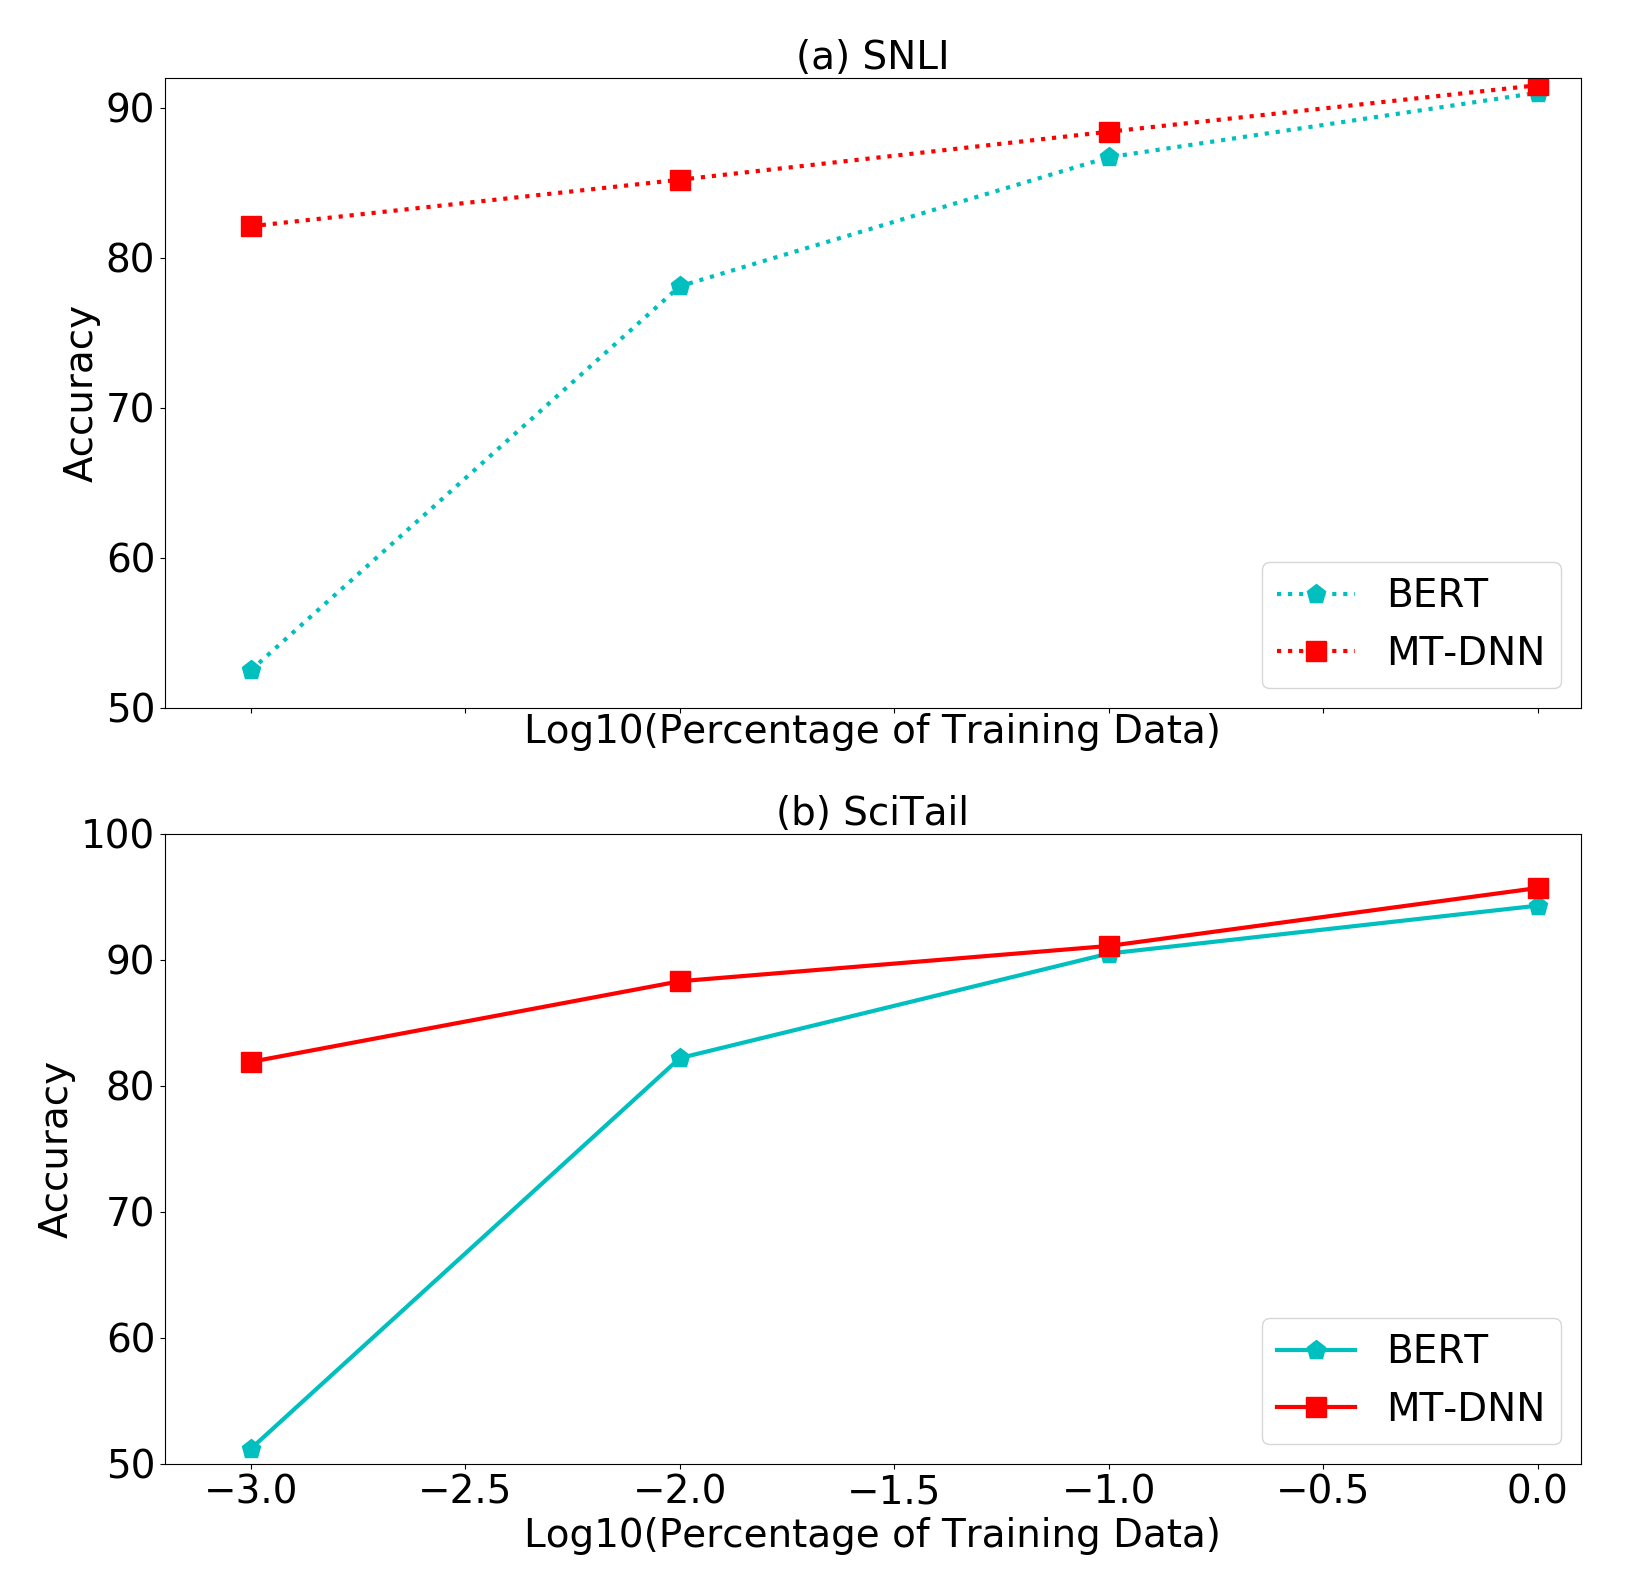
\includegraphics[width=0.5\textwidth]{fig/da.png}
    }   
    \caption{\label{fig:domain} Domain Adaption on SNLI and SciTail development datasets: Comparison of the shared embeddings. The X-axis indicates the amount of labeled samples used in finetuning models.}
\end{figure}
One of important criteria for building practical systems is robust and generalized to other tasks or new domains. This is because it is prohibitively expensive to collect labeled training data for new domains or tasks. Very often, we only have very small training data or even no training data, which hinders real-world applications. 

To evaluate the models using the above criteria, we perform domain adaptation experiments on SNLI/SciTail using the following procedure: 1) train a {\MNAME} on eight tasks in GLUE except WNLI \footnote{There are issues in this dataset as: https://gluebenchmark.com/faq.}; 2) use the shared layer weight as initiation for a new task, e.g. SNLI and SciTail. 3) finetune the model on these tasks and evaluate it. We denote this approach as \textbf{MT-DNN}. As a comparison, we use model initialized by BERT as a baseline, denoting \textbf{BERT}.

We split the training data of SNLI and SciTail, and randomly sample 0.1\%, 1\%, 10\% and 100\% of its training data. As a result, we obtain 4 sets of training data for SciTail, which includes  23, 235, 2.3k and 23.5k training samples. Similarly, we obtain 4 sets of training data for SNLI, which includes 549, 5.5k, 54.9k and 549.3k training samples.

Results on different amount of training data of SNLI and SciTail are reported in Figure~\ref{fig:domain}. We observe that our model pre-trained on GLUE via multi-task learning dominates the BERT baseline. With even a few training samples, e.g., 0.1\% (23 samples) of SciTail Training, our model achieves 81.9 in terms of accuracy (vs 51.2 obtained by the BERT baseline), indicating that the proposed model is more generalized and robust.  
%{\xiaodl{TODO: Add feature-based DA}}
% \noindent \textbf{Metrics:}
% We evaluate our model on the General Language Understanding Evaluation (GLUE) benchmark, which is a collection of diverse natural language understanding tasks. 

% Table~\cite{tab:datasets} summarizes the statistics of GLUE benchmark and its task formulation.
% The detailed description of each dataset is originally
% summarized in Wang et al. (2018):